\documentclass{article}
\usepackage{amsmath}
\usepackage{graphicx}
\advance\textwidth by1.4in\advance\oddsidemargin by-0.7in
\advance\textheight by1.1in\headheight 0pt\topskip 0pt\headsep 0pt\topmargin 0pt
\begin{document}
\thispagestyle{empty}
\begin{center}
  \large\bf Runtime Compiler(RTC) \\ 
  \large\bf By Rich Drake and James Foucar \\
  \bigskip
\end{center}


\section*{Tables of Contents}
\begin{itemize}
  \item 1. Introduction
    \begin{itemize}
      \item 1.1 What is RTC?
      \item 1.2 Motivation for RTC
      \item 1.3 Abilities of RTC
      \item 1.4 Implementation of RTC
    \end{itemize}
  \item 2. Usage
    \begin{itemize}
      \item 2.1 Using RTC as a user-defined initial condition
      \item 2.2 Using RTC as a library
      \item 2.3 The RTC language
        \begin{itemize}
          \item 2.3.1 Operators
          \item 2.3.2 Control Flow
          \item 2.3.3 Line Structure
          \item 2.3.4 Variables
          \item 2.3.5 Math
          \item 2.3.6 Strings
          \item 2.3.7 Printf
          \item 2.3.8 Comments
          \item 2.3.9 Unsupported Features
          \item 2.3.10 Examples
        \end{itemize}
      \item 2.4 Using RTC and APREPRO
      \item 2.5 Adding Runtime-bound functions
      \item 2.6 Recent Changes
      \item 2.7 Troubleshooting 
    \end{itemize}
\end{itemize}

\section{Introduction}

\subsection{What is RTC?}

RTC is an independent, self-contained library that compiles a string into
a set of in-memory data structures that can be executed. This gives users the 
ability to runtime-compile a small program, pass in arguments to the program, 
and execute this code all during runtime. If the client of RTC is getting this 
string from a file, the file can be changed, potentially causing different 
behavior in the client without the client having to be recompiled.

\subsection{Motivation for RTC}

RTC was created in order to provide users a way to express methods in the
input decks for physics codes. One common way which this ability is used
is for users to define the initial conditions for variables (density, 
temperature, etc) as a function of the x,y, and/or z coordinates of the 
entity (node, element, etc) whose property is being defined. This gives users
a more powerful way to define their initial conditions without requiring a
significant increase in the complexity of the input file parser. \\

\noindent
RTC is also useful for describing boundary conditions, source terms,
material properties, and any other independent variable. 

\subsection{Abilities of RTC}

RTC allows users to set up a function with any number of arguments. Argments
may be of the type int, float, double, or char. Arguments may be arrays or
scalars. Arguments can be passed in by reference or by value (one caveat is
that arrays must be passed by reference). Once RTC is notified of the names 
and types of a function's arguments, the body of a function (C-code packed into
a string) can be passed in and it will be compiled. The compiler will detect
any errors and provide the exact line at which the error occured. Errors are
returned to the user as a string. If the empty string is returned, then there
were no errors. At any point in time, the user can provide values for the
arguments they intend to pass into their RTC function. Once all the argument
values have been provided, the function can be executed. The function can
be indefinately re-executed with different argument values. 

\subsection{Implementation of RTC}

\begin{center}
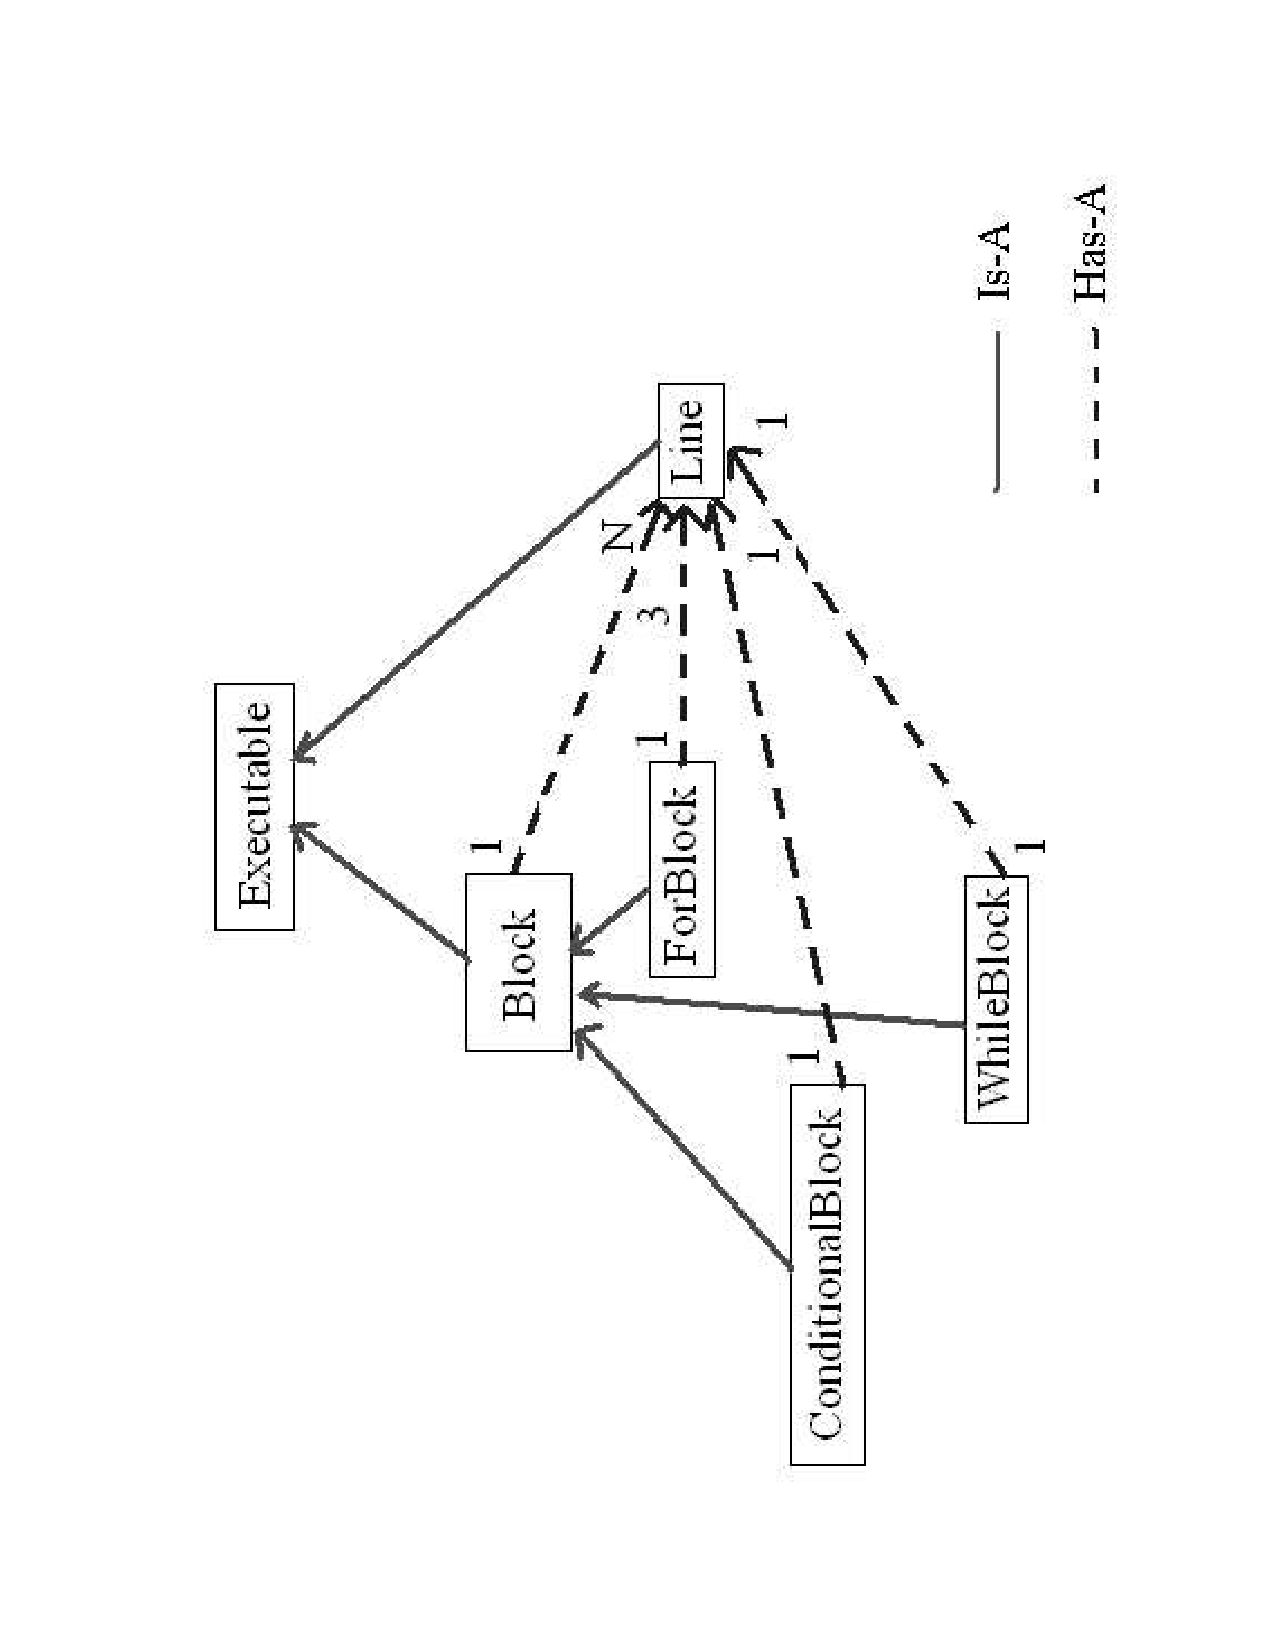
\includegraphics[scale=0.36,angle=270]{diag1}
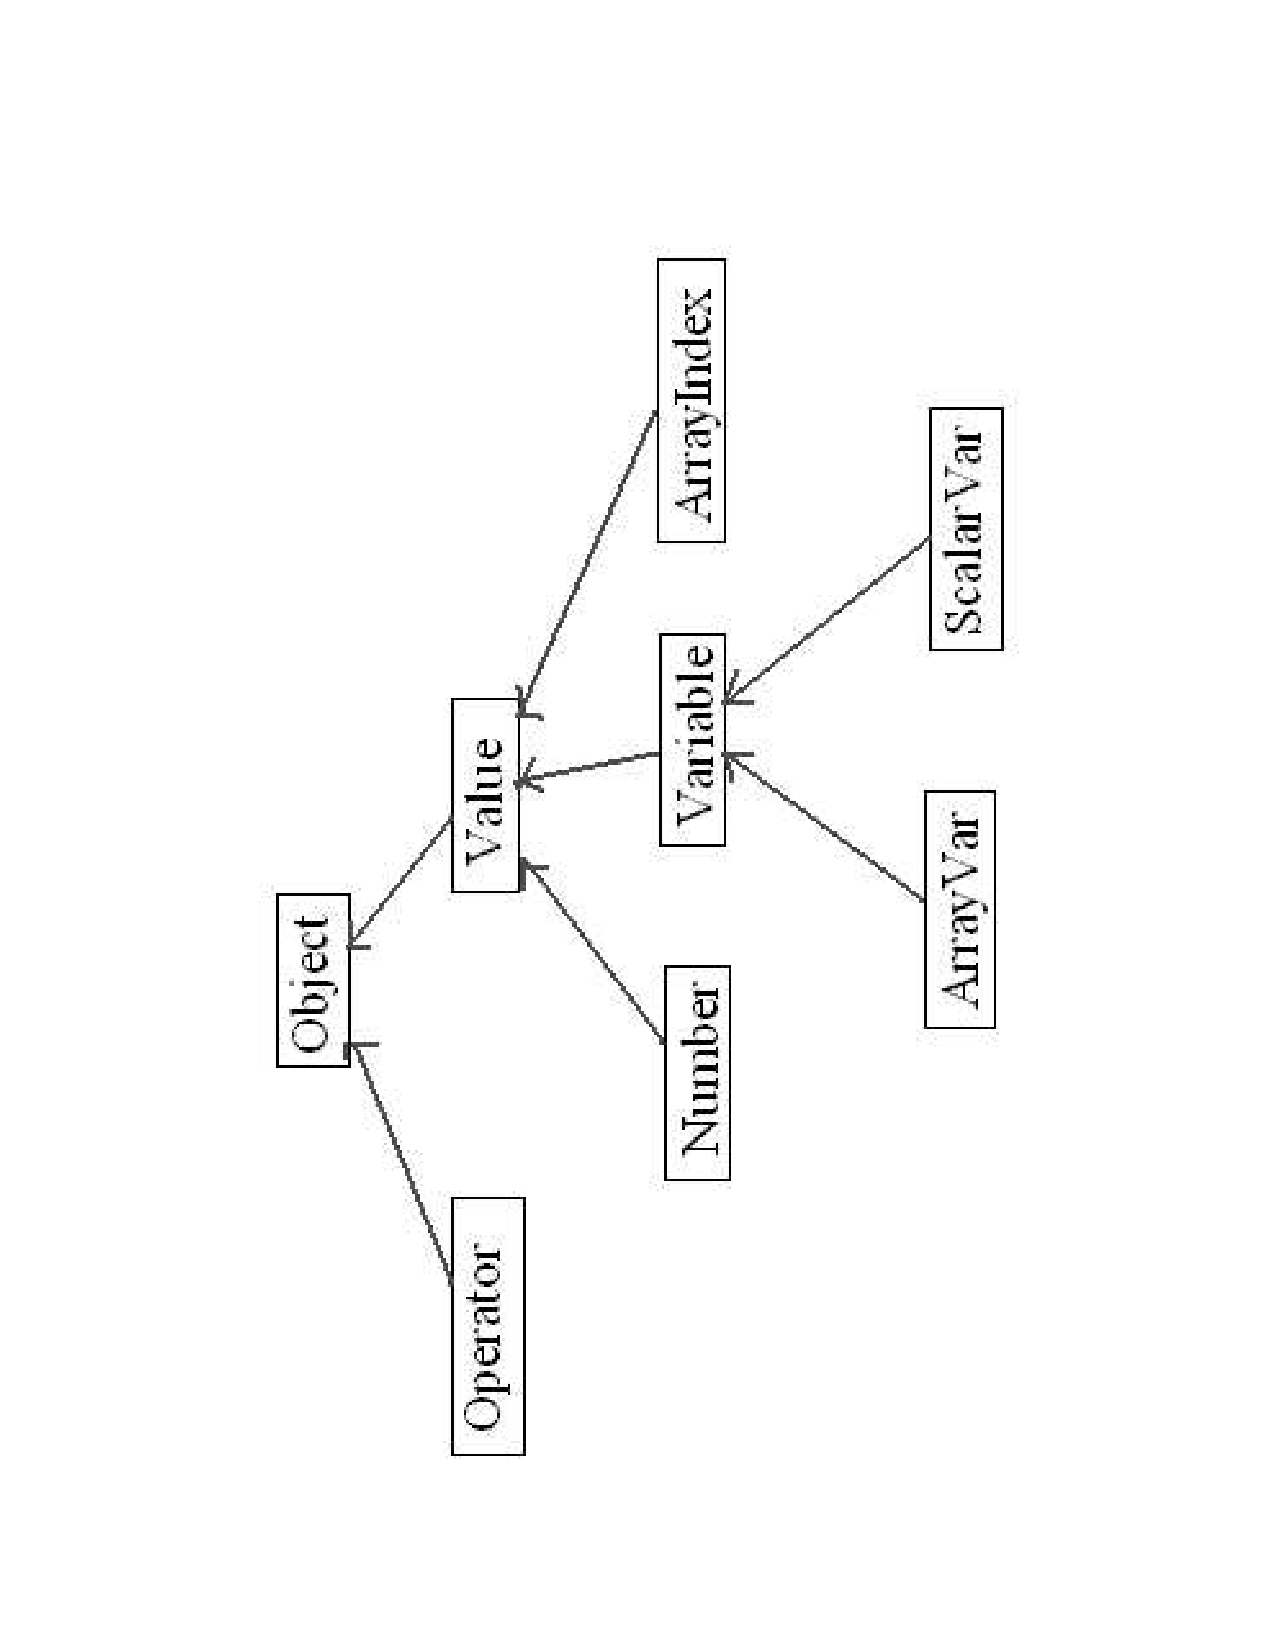
\includegraphics[scale=0.36,angle=270]{diag2}
\end{center}

\noindent
The first diagram shows how the code is organized. Each individual line is
compiled into postfix and stored into the Line class. The Block classes
contain a collection of lines. The second diagram shows how individual
entities found in a line are organized.

\noindent
The RTC library has many classes, but only a few of them are interesting.\\

\noindent
The Function class provides the user interface to the library. It also 
maintains the argument collection and ensure that all arguments are specified 
before compiled and that their values are filled before execution. When a 
function body is given to Function for compilation, it gets sent to 
Tokenizer for tokenization and the tokens are then given to NormalBlock so
it can create its subcomponents (lines and sub-blocks). Execution is simple;
the top NormalBlock is told to execute. See below for more on blocks.\\

\noindent
The Tokenizer class contains the first level of the parser. It transforms
a raw string into collections of Tokens. Tokenizer parser a string by looking
at runs of characters. For example, if the first character it sees is numeric,
the parser knows it has encountered a number and will enter a loop, grabbing
numeric characters until there aren't anymore and then creating a token with
the grabbed characters. The grammar of the C-language is loosely enforces by
a comes-after operation. After the type of a token is verified, we check that
this type of token may follow the type of token that preceded it. While this
system may not be quite as robust as using grammar trees, it is much easier
to implement and catches the vast majority of grammar mistakes. The Tokenizer
class also provides convenient ways of iterating through its tokens. \\

\noindent
The Block class is a parent to the many types of sub-blocks (WhileBlock,
ConditionalBlock, ForBlock, etc). A block represents all the executable
items (lines and subblocks) within a \{ and \}. A block knows all the 
varaibles that are available within its scope. During compilation, a block
creates its executable items by looking at the tokens it is given. For 
example, say the following string was given to library to compile:
{\ttfamily \begin{verbatim}
int i = 0;                      \\1 
int j = 0;                      \\2 
if (i == j) {                   \\3
  int a = 2;                    \\4
  print(j);                     \\5
  for( i = 0; i < 10; i=i+1) {  \\6
    j = j + 2;                  \\7
  }                             \\8
}                               \\9
print(j);                       \\10
\end{verbatim} }
\noindent
The top block would be a NormalBlock that would contain the entire function.
Its list of executable items would be \{line 1, line 2, a ConditionalBlock 
beginning at line 3, and line 10\}. The ConditionalBlock would contain its
condition statement $(i == j)$ and the executable items \{line 4, line 5,
and a ForBlock beginning at line 6\}. The ForBlock will contain its three
special statements: the initialization statement $i = 0$, the conditional
statement $i < 10$, and its post-processing statement $i=i+1$ and, of course,
its executable items: \{line 7\}. \\

\noindent 
During compilation, a block will iterate through the tokens. If it sees a 
block-opening statement (if, while, etc), it will create the appropriate
block and let the new block takeover. Once the new block returns, the original
block can assume that the new block iterated until it encountered a \} that
matched with its opening \{. This means that all executable items that follow
once again will belong to the original block. \\

\noindent 
Execution is different for each type of block. A NormalBlock simply executes
all its executable items in order. A ConditionalBlock executes its condition
statement first. If the result is non-zero, it then executes all its executable
items. \\

\noindent
The Line class is responsible for taking a collection of tokens and finding 
the meaning of the tokens. In other words, it converts a collection of tokens
into a postfix stack of operators and operands. The line class is able to find
any errors that the Tokenizer may have missed. A Line executes by processing
its postfix stack in a well known manner 
(see http://academics.tjhsst.edu/compsci/apcs/january/node3.html). 

\section{Usage}

\subsection{Using RTC as a user-defined initial condition}

To create a user-defined initial condition, somewhere in the definition of 
your physics, you'll need to do the following:

{\ttfamily \begin{verbatim}
user defined initial condition, varName [, block n m z ...]
"
 Function goes here. 
"
end
\end{verbatim} }

\noindent
The above will initial the variable corresponing to varName for blocks n,m,z.
If the block specification is left out, all blocks will be affected. 
Use coord[0,1,2] to access coordinates of the object whose initial condition 
is being defined. coord[0] gives the x-coord, coord[1] gives the y-coord, and
coord[2] gives the z-coord. For 2d, only coord[0,1] will work. Store the 
values for varName in the field array. If varName is scalar, use only field[0].
If varName is 3-dimensional, use field[0,1,2]. In other works, the coord array 
is your input and the field array is your output.\\

\noindent
An example may be the best way to illustrate the usefulness of runtime
compiled functions:

{\ttfamily \begin{verbatim}
user defined initial condition, density, block 5
" 
  field[0] = 100.0;
  if(coord[0] > 0.0){
    double distance = sqrt ((coord[0]^2) + (coord[1]^2) + (coord[2]^2));
    field[0] = field[0] + distance;
  }
"
end
\end{verbatim} }
\noindent
The above function first sets \texttt{field[0]} to a value of 100.0, then in 
the region of the domain where \texttt{coord[0]} exceeds 0.0 field is 
incremented by the distance from the origin. In this context \texttt{coord[0]} 
is the \texttt{X} coordinate, and the resulting evaluation will calculate a
constant value of \texttt{field[0]} in the negative half plane and a
monotonically increasing value of \texttt{field[0]} in the positive half plane.\\

\noindent
See section 2.3.7 for additional examples. 

\subsection{Using RTC as a library}

This section will describe how to use RTC in general. \\

\noindent
There is only one Function constructor and it takes a string and an integer 
argument. The string is the name of the Function, the integer is the number of
arguments the Function will take. For example:
{\ttfamily \begin{verbatim}
Function sampleFunc("sample", 2);
\end{verbatim} }
\noindent
This sets up the Function sampleFunc to take two arguments.\\

\noindent
Next, you must specify the type of each argument. You do this by calling the
addVar(string type, string name) method. It adds a variable of type type and
name name to the argument list for the function. For example:
{\ttfamily \begin{verbatim}
sampleFunc.addVar("int", "myint");
\end{verbatim} }
\noindent
This adds an integer named myint to the arg list for sampleFunc. It will return
false if it fails. Note: having whitespace in these arguments will cause an 
error to be generated. \\

\noindent
After you have specified the type and name for all of the arguments, you can
compile the body of the code. You do this by calling the addBody(string body)
method. It returns false if it fails. For example:
{\ttfamily \begin{verbatim}
sampleFunc.addBody(s);
\end{verbatim} }
\noindent
This compiles the program stored in the string s. \\

\noindent
After you have compiled, at some point, much later in the program if you wish,
you can fill the values or addresses of the arguments for the function. You
do this with the varValueFill, varAddrFill, and arrayAddrFill methods. These
methods return false if they fail. For example:
{\ttfamily \begin{verbatim}
sampleFunc.varValueFill(0, 10);
\end{verbatim} }
\noindent
This call would fill the first argument in the argument list with the value
10. Some things to note: notice that the first argument passed to varValueFill
is an integer. This integer is an index to the argument list of sampleFunc.
Also, varValueFill is only for arguments that you want to pass by value. If 
you want to pass by-reference, use the varAddrFill method. If you want to pass
in an array, use the arrayAddrFill method. \\

\noindent
Once you have added all the arguments, compiled the body, and filled all the
arguments, you are ready to execute the function. You do this using the 
execute() method. For example:
{\ttfamily \begin{verbatim}
sampleFunc.execute();
\end{verbatim} }
\noindent
This will run sampleFunc(). \\

\noindent
The following is a complete example use of the program.
Note: In order to keep the code clean, I avoid checking for errors, but I
highly recommend checking for errors after calling methods.
{\ttfamily \begin{verbatim}
//BEGIN
	Function factorial("factorial", 2);
	factorial.addVar("int", "fac");
	factorial.addVar("int[]", "intarray");

	//...

	int fac = 1;
	int* addr = &fac;
	int arraySize = 5;

	int* intarray = new int[arraySize];
	for (int i = 0; i < 5; ++i)
	    intarray[i] = i+1;

	factorial.varAddrFill(0, addr);
	factorial.arrayAddrFill(1, intarray, arraySize);

	string s = "for (int i = 0; i < 5; i=i+1) { \
		 	fac = fac * intarray[i]; \
		    }"; 

	factorial.addBody(s);

	factorial.execute();

	cout << "Factorial of 5: " << fac << endl;
//END
\end{verbatim} }


%% NOTE: this file is shared directly with the Alegra Users Manual
%% NOTE: this file is shared directly between the Alegra Users Manual and
%%       the RTC writeup in alegra/toolkit/rtcompiler/writeup.tex

\subsection{The RTC language}

The RTC language can be thought of as a small subset of the
C language with a couple minor modifications. 

\subsubsection{Operators}

The RTC language has the following operators that work exactly as they do in C
and have the same precedence as they do in C:
\begin{itemize}
  \item $+$  Addition
  \item $-$  Subtration
  \item $-$  Negation
  \item $*$  Multiplication
  \item $/$  Division
  \item $==$ Equality
  \item $>$  Greater than
  \item $<$  Less than
  \item $>=$ Greater than or equal to
  \item $<=$ Less than or equal to
  \item $=$  Assignment
  \item $||$ Logical or
  \item $\&\&$ Logical and
  \item $!=$ Inequality
  \item $\%$ Modulo
  \item $!$  Logical not
\end{itemize}

\noindent The following operators do not occur in the C language, but were added to the RTC language for convenience:

\begin{itemize}
  \item \begin{verbatim}^ Exponentiation \end{verbatim}
\end{itemize}


\subsubsection{Control flow}

The RTC language has the following control flow statements:

\begin{itemize}
  \item for( expr ; expr ; expr ) \{ ... \}
  \item while( expr )  \{ ... \}
  \item if (expr) \{...\}
  \item else if (expr) \{...\}
  \item else \{...\}
\end{itemize}

\noindent These control flow statements work exactly as they do in C
except that the code blocks following a control flow statement 
\textbf{MUST} be enclosed within braces even if the block only consists of 
one line.

\subsubsection{Line Structure}

The line structure in the RTC language is the same as that of C. Expressions
end with a semicolon unless they are inside a control flow statement.

\subsubsection{Variables}

Declaring scalar variables in RTC is done exactly as it is done in C except 
that only the following types are supported:

\begin{itemize}
  \item int
  \item float
  \item double
  \item char
\end{itemize}

\noindent For scalars, variables can be declared and assigned all at once. Both of the 
following approaches will work:

{\ttfamily \begin{verbatim}
int myVar = 9;

OR

int myVar;
myVar = 9;
\end{verbatim}
}

\noindent Arrays work a little differently in RTC than they do in C. There are
no \emph{new} or \emph{malloc} operators, instead the user may 
declare dynamically sized arrays in the same manner as statically sized 
arrays. Also, in C all the values of an array may be initialized at once by 
putting the values within braces. This is not supported in the RTC language.
Users will have to loop through the array and assign the values one by one.
For example:

{\ttfamily \begin{verbatim}
LEGAL:
   int ia[x*y];  //Note: in C this would not be legal for non-const x,y
   int ia2[3];

NOT LEGAL:
   int ia[3] = {1, 2, 3};
\end{verbatim}
}

\noindent Indexing arrays can be done using the index operator:
array[expr] = ...;

\noindent Bounds checking is done at run time. If the bounds of an array are exceeded, 
it will dump an error to stdout. 

\subsubsection{Math}

The following math.h functions are available in RTC:

\begin{itemize}
  \item asin(arg)  : returns the arc sine of arg
  \item acos(arg)  : returns the arc cosine of arg
  \item atan(arg)  : returns the arc tangent of arg
  \item atan2(y, x): returns the arc tangent of y/x
  \item sin(arg)   : returns the sine of arg
  \item cos(arg)   : returns the cosine of arg
  \item tan(arg)   : returns the tangent of arg
  \item sqrt(arg)  : returns the square root of arg
  \item exp(arg)   : returns the natural logarithm base e raised to the arg 
                     power
  \item sinh(arg)  : returns the hyperbolic sine of arg
  \item cosh(arg)  : returns the hyperbolic cosine of arg
  \item tanh(arg)  : returns the hyperbolic tangent of arg
  \item log(arg)   : returns the natural logarithm for arg
  \item log10(arg) : returns the base 10 logarithm for arg
  \item rand(arg)  : returns a system-generated random integer between 0 and RAND\_MAX using seed arg
  \item fabs(arg)  : returns the absolute value of arg
  \item pow(b, e)  : returns b to the e power 
                     (Note: the Exponentiation operator is available)
  \item j0(arg)    : Bessel function of order zero
  \item j1(arg)    : Bessel function of order one
  \item i0(arg)    : Modified Bessel function of order zero
  \item i1(arg)    : Modified Bessel function of order one
  \item erf(arg)   : Error function 
  \item erfc(arg)  : Complementary error function  (1.0 - erf(x))
  \item gamma(arg)  : returns $\Gamma(arg)$
\end{itemize}

\subsubsection{Strings}

The user may pass quoted strings as arguments to 
functions. Note: it may be necessary to escape-out the double quotes so that they
do not confuse the input-file parser. See printf section below for an example.

\subsubsection{Printf}

The RTC printf method is called just like its C counterpart. The first argument
is a quoted character string. This string will contain the \% symbol 
which will tell RTC to output the corresponding argument. The only difference
between RTC's printf and C's printf is that in RTC's version, a type character 
after the \% is unnecessary. For example, inside an RTC method
the following is appropriate:

{\ttfamily \begin{verbatim}
printf(\"One:% Two:% Three:% \", 5-4, 2.0e0, 'c');\n\
\end{verbatim} }

\noindent
Which would generate this output: One:1 Two:2 Three:c

\subsubsection{Comments}

The traditional C-comment mechanism may be used inside RTC
functions. Use /* to begin a comment and */ to end the comment.

\subsubsection{Unsupported Features}

Implementing the entire C-language was well beyond the intent of RTC. Features 
that were too difficult or did not add enough value have been left out. 
The following is a list of common C features that are unsupported in RTC:
\begin{itemize}
  \item There are no $++$ or $--$ operators. Use $i = i + 1$ instead of $++i$
  \item Structs
  \item Pointers
  \item Instant array initialization: int array[5] = {1,2,3,4,5};
  \item Case statements
  \item Casting
  \item Labels and gotos
  \item Function definition/declaration
  \item stdio
  \item Keywords: break, continue, const, enum, register, return, sizeof,
    typedef, union, volatile, static.
\end{itemize} 




\subsection{Adding Runtime-bound functions}

Runtime-bound functions are essentially a library of functions that are 
available to RTC functions. This library can be expanded or two ways. \\

\noindent
First, one could edit the Registrar.cc and RegistrarRTC.hh files
directly. In RegistrarRTC.hh you would declare a new class that is a 
sub-class of the RTBoundFunc class. You need the contructor of this class
to contruct the parent class (RTBoundFunc) with the name of the function
and the number of arguments the function will expect. An optional third
argument specifies whether this function should be optimized. The compiler
will try to optimize functions that have constands for all their arguments.
For example, $\sin(4.5)$, would be replaced at compile time with the result 
of this call. However, certain functions, like print(x) should not be
optimized. This is what the optimization argument is for. Here is an example
of what the declaration of a new Runtime-bound function should look like:
{\ttfamily \begin{verbatim}
class Example : public RTBoundFunc
{
  public:
    Example() : RTBoundFunc("my_func", 2) {}
 
    double execute(Value**);
};
\end{verbatim} }
\noindent
Once you have your new Runtime-bound declared, you must provide the definition
of its execute method and register it with the Registrar class, the class that
contains all callable Runtime-bound functions. To achieve this, open the 
Registrar.cc file. Go to the Registrar::setup\_standard\_functions() method.
In this method, somewhere inside the ISINIT if-block, add the following
line:
{\ttfamily \begin{verbatim}
FUNCTIONS[Example().name()] = new Example();
\end{verbatim} }
\noindent
Providing a definition for the execute method is tricky. The input argument
to this method is an array of Values. The value interface is located in
the file ValueRTC.hh. You are allowed to ask these values for their type
and can set or ask for their values. For example, say we wanted our Example
rtbound function to assume its first argument is an array and to fill this
array with the value of the second argument and to return the value of the
second argument. Here is what that definition would look like:
{\ttfamily \begin{verbatim}
double Example::execute(Value** args) 
{
  assert(args[0]->getObjectType() == ArrayVarOT);

  //fills the array in args[0] with the value of args[1]
  for (int i = 0; i < args[0]->getSize(); ++i) 
    args[0]->setArrayValue(args[1]->getValue(), i);

  return args[1]->getValue();
}
\end{verbatim} }
\noindent
Notice that it might be wise to do some type checking at the top of the 
method. As far as I could tell, there was no simple way of doing argument
type-checking at compile time. \\

\noindent
The second way to expand the library is create a new RTBoundFunc subclass in
your own source file. During initialization time, you can call 
Register::register\_function(...) and add your new RTBoundFunc without having
to modify the RTC code. This approach is probably better if your RTBoundFunc
would cause dependencies if it relied on special function calls. 

\noindent
Once you've registered your RTBoundFunc, you should be able to call it just 
like any other function ($\sin$, $\cos$, etc).

\noindent
There is a new type of runtime-bound function available to users: functions
without a fixed signature, like printf. In order to have your RTBoundFunc be
a variable signature function, there is an optional fourth argument for the
constructor. See the implementation of the class Printf in RegistrarRTC.hh and
Registrar.cc for an example.

\subsection{Recent Changes}

\begin{itemize}
  \item printf - See printf subsection (Added 3/8/06)
  \item comments - See comments subsection (Added 3/8/06)
  \item variable signature runtime-bound functions - See end of runtime-bound 
        function section. (Added 3/8/06)
\end{itemize}

\subsection{Troubleshooting}

The easiest way to figure out why your function is not running is to look at
the error messages if any are generated. Most error messages will tell you the
line of the problem. In general, most of the methods on a Function object that 
the user would be calling will return a bool. If the bool is false, that means
there was an error. Error messages can be retrieved by calling the getErrors() 
method. So, the general form of your usage of the program should resemble the 
following:
{\ttfamily \begin{verbatim}
if (!someFunctionObject.someMethod()) 
  cout << functionObject.getErrors();
\end{verbatim} }

\noindent
If you are really having trouble with an error or bug, feel free to email me
for help at: \begin{verbatim} jgfouca@sandia.gov \end{verbatim}

\end{document}
